\begin{tikzpicture}[every node/.style={inner sep=0,outer sep=0}]

	\node [anchor=north east] (img1) at (-0.03\textwidth,0) {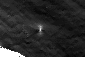
\includegraphics[width=.4\textwidth]{05_ergebnisse/ergDiskussion/figures/pickel}};
	\node [below=0.2cm of img1, align=center] {Ausschnitt von Keramikobjekt 1 \\ aus Abbildung \ref{tikz:abbAbleitungRegistrierungSpiegel}};
	\node [anchor=north west] (img2) at (0.03\textwidth,0) {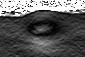
\includegraphics[width=.4\textwidth]{05_ergebnisse/ergDiskussion/figures/delle}};
	\node [below=0.2cm of img2, align=center] {Ausschnitt von Keramikobjekt 2 \\ aus Abbildung \ref{tikz:abbAbleitungRegistrierungSpiegel}};
	
\end{tikzpicture}
\caption[Erkennbare Oberflächendefekte durch deflektometrische Registrierung]{Erkennbare Oberflächendefekte durch Ableitung der deflektometrischen Registrierung. Linkes Teilbild: Oberflächenpickel, Rechtes Teilbild: Delle in der Oberfläche}